\documentclass[portfolio.tex]{subfiles}
\begin{document}
	\Chapter{Week 7}{Digging Deeper into Vue}
	\section{Weekly Content}

	\subsection{Component Registration}
		\label{vue-component-registration}
		Components can be registered in three ways: Global, Local, and Single FIle.
		\subsubsection{Global Registration}
			Global Components are available everywhere within the Vue Application.  A global component can be registered with the following syntax:\\

				\noindent \textbf{Vue.component('my-component', \{ \textit{ENTER COMPONENT DETAILS... \}})}\\

				 \noindent This means that anywhere within the HTML, a new component can be registered using $<$my-component$>$.


		\subsubsection{Local Registration}
			On the other hand, locally registered components can only be used within the scope in which they are registered. For example:\\

			\begin{lstlisting}
<script>
	var ComponentA = {...};

	new Vue({
		el: '#app',
		components: {
			component-a: ComponentA,
		}
	})
</script>
			\end{lstlisting}
		\bigbreak

		Now within the Vue app, the component can be used as component-a. However if we were to declare a second component component-a would not be available inside:\\

		\begin{lstlisting}
<script>
var ComponentA = {...};
var ComponentB = {
	template: '  <div><component-a>  <!-- THIS WON'T WORK! --> </component-a></div>'
}

new Vue({
	el: '#app',
	components: {
		component-a: ComponentA,
	}
})
</script>
		\end{lstlisting}

		\subsubsection{Single-File Components}
			Single-file components are almost a combination of global and local components. Single file components are stored in a \textbf{.vue} file and are  available anywhere within the Vue application but only if that vue file is imported. The following syntax can be used within the a JavaScript portion to import a component: \textbf{import ComponentName from './ComponentName.vue'}.\\

			Within the file, there should be three tags $<$template$>$,$<$script$>$ and $<$style$>$. template holds the template information such as HTML, or custom components. script holds all the custom JavaScript. It also is where the component is initialised using an object with fields such as data, name, methods, etc... style holds all the relevant CSS. The scoped modifier can be used to ensure the styles within this tag only apply to this component, even if other tags have the same classes.\\

			The trade-off for the ease-of-use of single file components is the complexity of the setup. These cannot simply be inserted into regular HTML and require the use of Module Build systems like webpack/npm, etc.\\

			Here is an example of a basic component:

			\begin{lstlisting}
<template>
	<CustomWrapper>
		<h1 class="title"> {{ title }}  </h1>
	</CustomWrapper>
</template>

<script>
	import CustomWrapper from './CustomWrapper.vue'

	export default {
		name: "MyComponent",
		components: { CustomWrapper },
		data() {
			return {
				title: "My Title",
			};
		},
	}
</script>

<style scoped>
	.title {
		color: red;
		font-weight: bold;
	}
</style>
			\end{lstlisting}
	\subsection{Props, Custom Events, Dynamic \& Async Components}
		For these topics please see \ref{task4} where I have discussed them already.

	\section{Practical Tasks}
		\subsection{Task 1}
			Within my project I have opted to use single-file components. Especially when building a fully vue-focused application, I find this to be the cleanest and most organized way of creating components. \\

		\subsubsection{Source Code}

		Here are two examples of Single File components I have created:\\

		\seqsplit{https://github.com/BrandonMurch/SIT120/blob/021a2694432d61e32c9fba191ee7579c2dfdb955/Assignment\%201/updated-proof-of-concept/tend/src/App.vue}\\

		\seqsplit{https://github.com/BrandonMurch/SIT120/blob/main/Assignment\%201/updated-proof-of-concept/tend/src/components/TheExplorePlants.vue}\\

		For a full list, see:\\
		\seqsplit{https://github.com/BrandonMurch/SIT120/tree/main/Assignment\%201/updated-proof-of-concept/tend/src/components}
		\subsubsection{Screenshot}
		I have included a picture of my project so far with different coloured squares highlighting different components.

	\begin{center}
		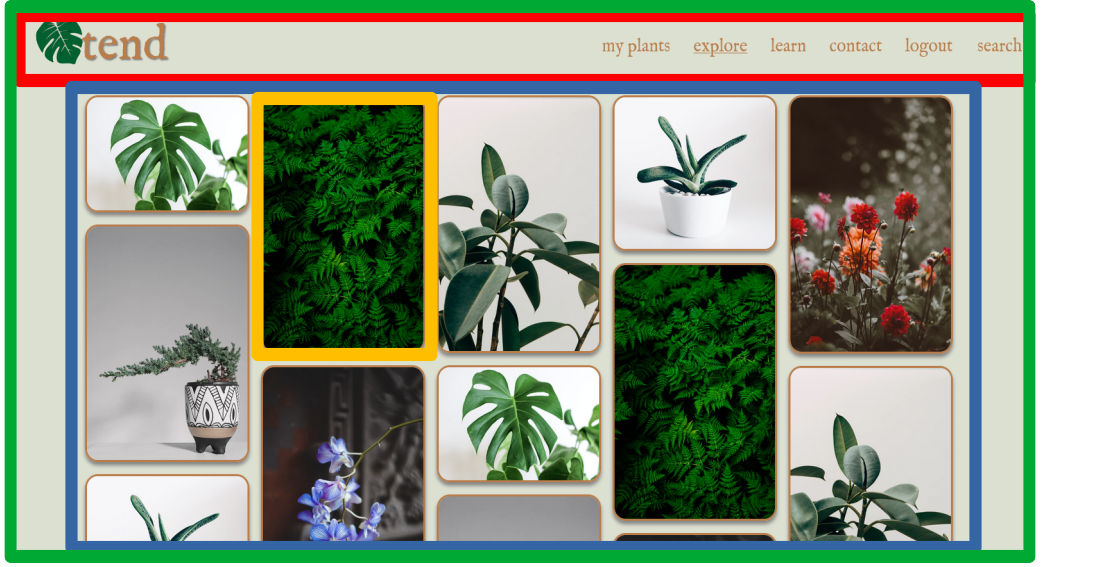
\includegraphics[width = 14cm]{components-example.png}
	\end{center}

	\subsection{Task 2}
		I have used props throughout my project to increase the reusability of my components. This allows me to create one component, which can be reused for many elements.\\

	\subsubsection{Screenshot}
	This screenshot shows the same component (CardImage) but which contains two different images that were passed in using props.

	\begin{center}
		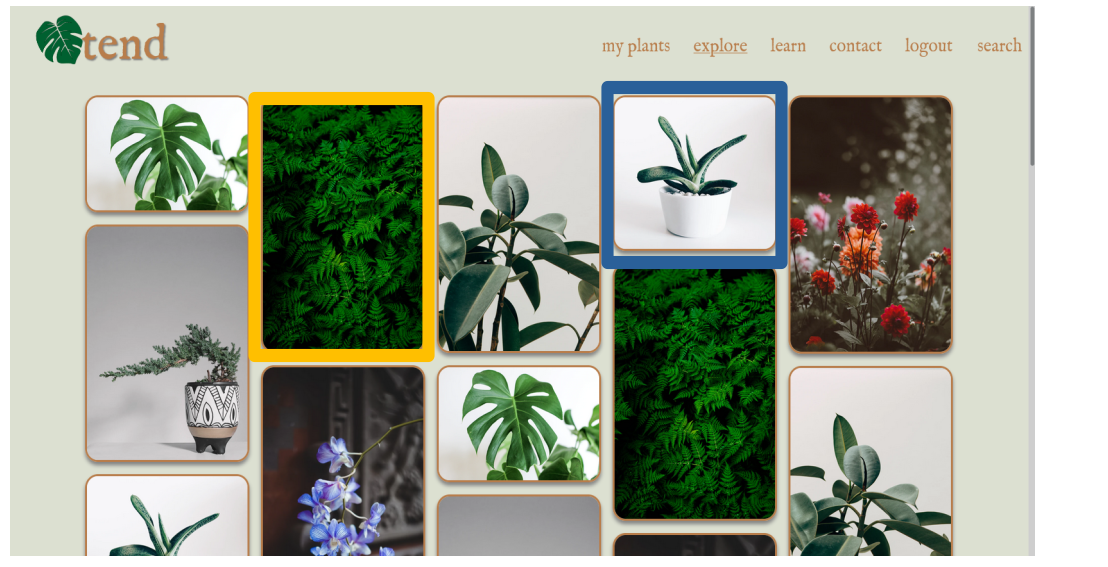
\includegraphics[width = 14cm]{props-example.png}
	\end{center}

	\subsubsection{Source Code}

		\seqsplit{https://github.com/BrandonMurch/SIT120/blob/021a2694432d61e32c9fba191ee7579c2dfdb955/Assignment\%201/updated-proof-of-concept/tend/src/components/CardImage.vue}\\
		\seqsplit{https://github.com/BrandonMurch/SIT120/blob/021a2694432d61e32c9fba191ee7579c2dfdb955/Assignment\%201/updated-proof-of-concept/tend/src/components/ImageGallery.vue}

	\subsection{Task 3}

	One of the many custom events I have created in my application is the moreImages event. This application is created by the ImageGallery component. When the user scrolls to the bottom of this component, the image gallery emits the call for more images. This allows the parent node to provide more images if it is possible.

	\subsubsection{Github Link}

	\seqsplit{https://github.com/BrandonMurch/SIT120/blob/021a2694432d61e32c9fba191ee7579c2dfdb955/Assignment\%201/updated-proof-of-concept/tend/src/components/ImageGallery.vue}

	\subsubsection{Screenshot}

	\begin{center}
		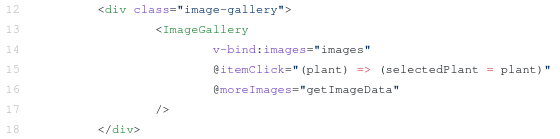
\includegraphics[width = 14cm]{custom-event-example.png}
	\end{center}

	\subsection{Task 4}
		I used a named slot within the DropDown component. In the future, this will allow me to specify multiple components all within the one drop down menu.

	\subsubsection{Github Link}

		\seqsplit{https://github.com/BrandonMurch/SIT120/blob/021a2694432d61e32c9fba191ee7579c2dfdb955/Assignment\%201/updated-proof-of-concept/tend/src/components/DropDown.vue}
	\subsubsection{Screenshot}

	\begin{center}
		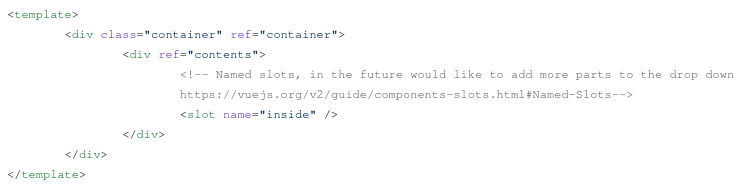
\includegraphics[width = 14cm]{slots-example.png}
	\end{center}

	\section{Project}
	\subsection{What I accomplished this week}
		This week I have completed the MyPlants portion of the website. I have allowed the user to update plant settings, see notifications and create new plants.

	\subsection{What I would like to accomplish next week}
		Next Week I would like to complete the "Learn" portion of tend, and populate it with a series of fake articles, questions and answers. This should take me about 5 hours to complete and polish. The following week should be all about fully polishing my website, and adding in small touches.

\pagebreak
\end{document}